Before starting the project several areas were investigated to understand the North Atlantic Right Whale better and to see what others had done to perform classification on images, and what preprocessing techniques could be used.

\subsection{North Atlantic Right Whales}
Through the last decades the North Atlantic Right Whale have become an endangered whale species \cite{NOAA}. The North Atlantic Right Whale have been added to the list of animals under the protection of ESA\footnote{The Endangered Species Act} in 1931. The problem of this convention is that both Japan and the Soviet Union did not sign the agreement. Consequently, meaning that commercial whaling of the North Atlantic Right Whale to a large extend continued until 1949 where the whale species came under the protection of the International Convention for Regulation of Whaling. 
This convention deals with regulation of commercial whiling, but does not prohibit commercial whaling. 
This lead to an over-utilization of whaling in its primary habitat. The result of the commercial over-utilization meant that in 1970 the whale were determined to be in danger of extinction. 
Further, over the next decade, it has been added to both Endangered Species Convention Act, and designated the Marine Mammal Protection Act (MMPA) as Depleted.

In 2015 it have been estimated that there is fewer than 500 individual whales left. Nowadays, fishing of the whale is completely prohibited, but there are still a number of threats for the survival of the North Atlantic Right Whale.
These threats are:
\begin{itemize}
	\item Ship collisions 
	\item Entanglement of fishing gear
	\item Habitat Degradation 
	\item Contaminants
	\item Climate/Ecosystem changes
	\item Disturbance of whale-watching activities
	\item Noise from industrial activities
\end{itemize}
To counter these threats and recover the population of the North Atlantic Right Whale a recovery plan was established in 1991 \cite{NOAARecovery}. 
The goal of this plan is to downgrade the status of the whale species from endangered to threatened.
To accomplish this goal the recovery plan states seven major recommendations to:
\begin{enumerate}
	\item Reduce or eliminate injury or mortality caused by ship collision
	\item Reduce or eliminate injury and mortality caused by fisheries and fishing gear
	\item Protect habitats essential to the survival and recovery of the species
	\item Minimize effects of vessel disturbance
	\item Continue international ban on hunting and other directed take
	\item Monitor the population size and trends in abundance of the species
	\item Maximize efforts to free entangled or stranded right whales and acquire scientific information from dead specimens
\end{enumerate} 

This paper contributes to number 6, concerning monitoring size and trends.

\subsubsection{Monitoring the population}
The task of monitoring population consist of the following major tasks:
\begin{itemize}
\item \textit{General Monitoring of population.}
\item \textit{Monitoring of habitats.}
\item \textit{Emergency response.}
\end{itemize}

The protection of the whales species is regulated worldwide but Coordinated nationally, and responded to locally. This requires a lot of knowledge sharing in order the coordinate the effort. The problem here is that the different individual local institutions can make better decisions and reduce their effort by having the shared knowledge of all the individual institutions.
Further, as it is now only a few people who has the skill needed to actually identify individual whales.

For this reason, the a photo-identification database have been created. This database contains a set of images of each individual North Atlantic Right Whale. 
These images can then be used by the local institutions to compare which whales they have seen with the database, thereby ease the identification of a whale and make sure that each different institute talk about the same whale when sharing knowledge. Besides the images it contains a location/sighting history and a log.
The problem that still remains is the accurate identification of a whale. Even though it is possible to browse through the database and compare the observed with the entries in the database unique identification is both time consuming and inaccurate from the non experts.
Even if the identification have to go through the experts, it will be so time consuming that local institutions will have to wait long periods of time for an answer.
Since time is a critical factor in the protection of the whales this would cause big problems.

\subsubsection{How to recognize the whales}
It is a common technique to use image recognition to identity unique whales, many species has physical markings where it is possible to identity individual whales based on those markings. The North Atlantic Right Whale is no different. Figure \ref{fig:whale-collosity} shows the most important physical markings for the whales, it highlights some of the areas where unique characteristics can occur, while the white callosity in the middle is the most significant to look at \cite{neaq:whale-identity}. Besides the callosity other marks can be used to identify the whales:

\begin{itemize}
	\item Crenelations along the lower lip (also called lip “ridges”)
	\item Distinctive white patches on the belly and chin
	\item A dip or depression in the rostrum that can be seen in profile
	\item Erosion of the callosity in the front of the bonnet refereed to as “tooth decay”
	\item Flukes that curve upwards as the whale dives
	\item White blow holes
	\item White fluke tips
	\item Gray lines behind the blow holes
	\item Divots in their backs
	\item White scars from a host of causes (including past entanglements in fishing gear, ship strikes, attacks by killer whales or false killer whales, skin lesions, and other unknown causes)
\end{itemize}

Some of these identifying marks can be inherited from a whales parents, while other markings are acquired through the whales life, for instance scars \cite{neaq:whale-identity-markings}. 

To correctly identify a whale, it is therefore needed to isolate these unique markings and compare them in the images. 

\begin{figure}
	\centering
	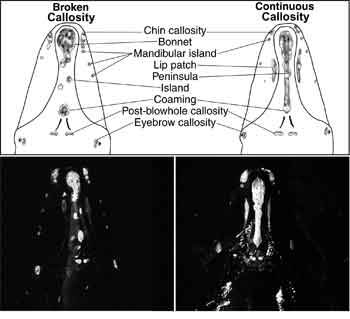
\includegraphics[width=\linewidth]{Images/callosity_comparison}
	\caption{Unique physical characteristics for North Atlantic Right Whales. Source: \cite{neaq:whale-identity}}
	\label{fig:whale-collosity}
\end{figure}

\subsection{Classification of images}
It was known beforehand that using Machine Learning algorithms could be used to classify images. What needed to be answered was which algorithms and techniques could be used for image recognition. 

The project is basically a facial recognition for whales, so research about how facial recognition systems work and what algorithms they use were done. Searching for articles, there are many implementations using different machine learning techniques, however some algorithms are more frequent than others. For instance the lecture from the CMU\footnote{Carnegie Mellon University} \cite{lit:nn1} explains how to use neural networks for facial recognition and argues that it is one of the best techniques to use. Likewise the article from \cite{lit:nn2} describes how a specific implementation of a neural network, called Convolutional Neural Network is working exceptionally good on recognizing and classifying images. 

Other algorithms which seem to have noteworthy results is the Random Forest, which are used in the following articles \cite{lit:rn1} and \cite{lit:rn2} both have good results and the Support Vector Machine algorithm is used in these articles \cite{lit:svm1} and \cite{lit:svm2} also solves the problem sufficient.

Many other articles mention these algorithms as some of the best for doing facial recognition, which leads to the assumption that they would work well for doing the image recognition needed to classify the individual whales, since there are unique markings on the faces of human beings and on the whales.

%% Facial Recognition

% Neural Network
% - (1) http://web.archive.org/web/20030621155420/http://www-2.cs.cmu.edu/~tom/faces.html
% - (2) http://deeplearning.cs.cmu.edu/pdfs/Lawrence_et_al.pdf

% Random Forest 
% - (3) http://www.security.iitk.ac.in/contents/publications/mtech/VidyutGhosal.pdf
% - (4) https://kbsg.rwth-aachen.de/~schiffer/bib/icpr2008rff.pdf

% SVM
% - (5) http://cbcl.mit.edu/publications/ps/iccv2001.pdf
% - (6) http://papers.nips.cc/paper/1609-support-vector-machines-applied-to-face-recognition.pdf

\subsection{Preprocessing images}
\label{sec:litterature}
As mentioned in Section \ref{sec:descr-of-data} the individual data entries has varying and huge dimensions. 
This means that it will be necessary to reduce their dimensions. 
Downscaling the images is one of the easiest ways to reduce the dimensions.
The problem with reducing the dimensions through scaling, is that the whale is a relatively small part of the images. Figure \ref{fig:scale} shows one of the original images from the dataset and the same image downscaled to 45x30px. As seen from the figure the whale is nearly non existing in the new scale. The whale on the downscaled image is spanning over two pixels.
Further as the water is without information about the whale using computational time on processing it is unnecessary.

\begin{figure}
	\centering
	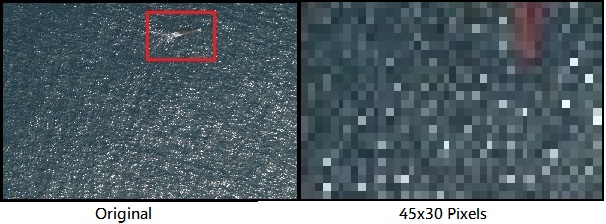
\includegraphics[width=\linewidth]{Images/scale}
	\caption{One picture from the data marked with a red square around the whale, and on the left the same image, downscaled to 45x30px}
\label{fig:scale}
\end{figure}

Therefore, removing the water would be another way of reducing the dimensions while maintaining information about the whale.

Leow Wee Kheng suggest a number of way that could be adopted for doing so \cite{backgroundRemoval}.
First, and easiest is to subtract the background from the image by:
\begin{figure}[H]
\begin{equation}
D(x,y) = |I(x,y) - P(x,y)|
\end{equation}
\caption{where \emph{D} is the Delta, \emph{I} is the image and \emph{P} is the background}
\end{figure}

After the subtraction colors in the delta \emph{D} is distorted, to get the original pixels back Kheng suggest the following:

\begin{figure}[H]
\begin{equation}
F(x,y) = \left \{
\begin{tabular}{cc}
$I(x,y)$ & $if D(x,y) > \Gamma$ \\
$B$      & $otherwise$
\end{tabular}  
\right \}
\end{equation}
\caption{Where \emph{F} is the foreground, \emph{I} is the original image, $\Gamma$ is a threshold and \emph{B} is the color wanted instead of the background}
\end{figure}

However this approach require the background to be known. For this problem domain each image have an unknown background.

Another suggested approach is to group pixels using k-means clustering\footnote{A description of clustering with K-means can be found in \ref{sec:methodology}}.

This approach have the advantage of adjusting to the individual images and their specific lighting conditions. Further it is possible to use without having any knowledge of what is background and foreground. 
In extend, clustering is flexible and can use features as well as pixel values.
For instance is it possible to combine this approach with the background modelling approach from \cite{backgroundRemoval}.
  
Background modeling works by looking at distribution of colors. Figure \ref{fig:pixeldistribution} shows a sample distribution from one of the images in the dataset. The figure shows that there are two main peaks in the distribution. One at around 0.2 the other at around 0.4. 
These peaks can be used to filter out different aspects of the images. This knowledge can be used as a feature to split values into different clusters.
 
\begin{figure}
\centering
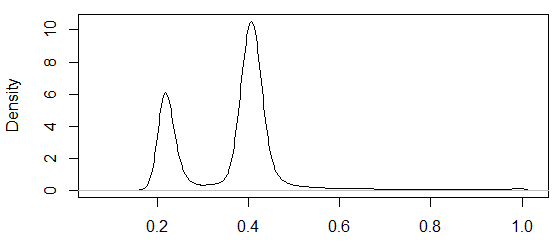
\includegraphics[width=\linewidth]{Images/Distribution}
\caption{Density plot of image pixels. The x-axis is different values for a pixel and the y-axis is the density of in the distribution of this value}
\label{fig:pixeldistribution}
\end{figure}